\subsubsection{\stid{2.10} PROTEAS-TUNE - Bricks} 

\paragraph{Overview}
We have developed a source-to-source structured grid data framework (``texttt{Bricks}'')
  to address the growing gap between memory and computational performance 
  on pre-exascale systems.
The approach uses standard \texttt{C++} code to express stencil loops, for example, 
  then transforms the code to use a different memory alignment and ghost
  zone region to optimize memory and communication performance specifically
  for that kernel~\cite{P3HPC_Bricks,zhao2019,zhaoMPI2019}.
This also provides an opportunity to inject architecture-specific code
  transformations, that can take advantage of SIMD/SIMT instructions, threading,
  virtual memory layouts, and specific parameters that are needed
  for each platform’s optimal performance.
This is a powerful paradigm for having both a correct legal code base 
  using standard tools and, in combination with the autotuning tools previously described,
  the ability to achieve portable performance on many different 
  platforms with auto-generated code transformations.

\paragraph{Key Challenges}
\texttt{Bricks} require three primary ingredients for performance portability:
\\
(1) \textit{Stencil kernel metadata} - For stencils, this includes stencil radius,
  dimensionality, neighbor dependences, and other memory access patterns.
  For example, for communication, the optimal layout depends on the
  extent of stencil corner coupling and symmetry or reuse.
For other kernels, it can involve making sure certain directions are contiguous,
  as in 1D FFTs or operators on neighboring vector components.
\\
(2) \textit{Transformation profitability model} - based on the architecture
  characteristics and benchmarks, determining what transformations could
  improve overall throughput, not just maximize flops or bytes moved. 
  This can also be explored using roofline models, auto-tuning, 
  communication-avoiding techniques, etc.
\\
(3) \textit{Back-end optimizations and benchmarks} - knowing what 
  architecture-specific transformations achieve the best roofline performance, 
  and how to isolate and compare those with a known benchmark problem. 
For example, if there
  are special hardware capabilities, like vector \textit{shuffle}, 
  or OS support for memory \textit{mmap} or \textit{prefetch}, that are required to obtain
  peak performance.

\begin{wrapfigure}{r}{0.35\textwidth}
\begin{center}
  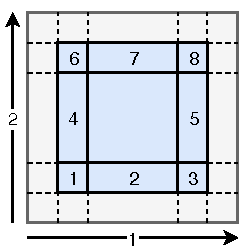
\includegraphics[trim=3mm 5mm 3mm 8mm,width=.33\textwidth]{projects/2.3.2-Tools/2.3.2.10-PROTEAS-YTUNE/Bricks-mpi-parts.pdf}
\end{center}
  \caption{\texttt{Bricks} can be used to map memory onto regions that
  eliminate ghost zone packing and MPI message count (2D example).}
\end{wrapfigure}

\paragraph{Solution Strategy}
With \texttt{Bricks}, we have developed a data layout library, code 
  generator, and communication primitives for both stencil computations and ghost zone communication.
Recent trends in computer architecture that favor computation over data 
  movement incentivize high-order methods and lower-precision data.
Paradoxically, high-order codes can be challenging for compilers/optimization 
  to attain high performance due to large amounts of intermediate data that exceeds available temporary storage.
\texttt{Bricks} enable high performance and make fine-grained data reuse and 
  memory access information known at compile or run-time.
Integration with autotuning attains performance that is close to Roofline
  performance bound for both manycore CPU and GPU architectures.

In addition, we have used our \texttt{Bricks} source-to-source transformation technique to 
  eliminate the cost of MPI packing/unpacking on CPUs and GPUs, which 
  improves strong scaling for block semi-structured applications, is 
  performance-portable, and is directly relevant to applications with many 
  DoF’s per grid point (such as in combustion and multi-physics codes). 
This is because for most stencil codes, strong scaling is
  limited by the communication of ``ghost zone'' values or exchanged between
  processors and nodes, which is required for iterative algorithms or time
  integrators. 
Typically, this means each MPI rank requires ``packing'' before sending – copying a 
  subset of local arrays into an MPI message buffer – and then ``unpacking'' 
  (copying buffers to array subset) after receiving data. 
These operations on the ghost zone ``skin'' can introduce significant latency 
  and is a blocking operation that, in the limit of strong scaling, 
  cannot be hidden by overlapping communication and computation. 
We have eliminated un/packing, and also introduced a novel technique on CPU to
  significantly reduce the number of messages, using an indirect mapping 
  of memory to MPI buffers. 

\paragraph{Recent Progress}
We have recently extended  \texttt{Bricks} to 
  incorporate run-time information on stencils, and use JIT (just-in-time) compilation to
  dynamically generate, compile, and link optimized kernels.
We have also extended the approach to 6D computations with mixed FFT and stencil
  calculations, such as are seen in Fusion science.
This required us to evaluate data types (real, complex) and precision (double, single) in the 
  context of different architectures’ performance-optimal parameters such as vector lengths
  and page/cache size.
We have extended SIMD code generation to achieve performance portability
  for high-order stencils for both CPUs with wide SIMD units (Intel Knights Landing and later 
  generations, ARM SVE) and GPUs (NVIDIA Ampere, AMD MI100, and Intel Gen11).  
We have demonstrated compatibility with standard \texttt{C++} and most major GPU
  programming models, including CUDA, HIP, DPC++ / SYCL, and OpenCL.

\paragraph{Next Steps}
For FY22, we are extending \texttt{Bricks} to other
  application patterns, including block-structured AMR, multigrid solvers,
  and systems of sparse and block-sparse (non-)linear systems.
For these, the primary focus will be on investigating the profitability
  models, code transformations, and auto-tuning the kernels.
As more diverse architectures and benchmarks become available within 
  the ECP program (AMD GPU, Intel GPU, NVIDIA Ampere), we will develop 
  transformations that provide better performance portability.
We will be building up to portable \textit{application} performance 
  and load balancing; this is a complex trade-off between all kernels in
  a given code, and will be very application- and architecture-dependent.

